\documentclass{article}
\usepackage{mathrsfs}
\usepackage{amsmath}
\usepackage{amsthm}
\usepackage{amssymb}
\usepackage{graphicx}
\usepackage{color}
\usepackage{float}
%\include{macros}
%\usepackage{floatflt}
%\usepackage{graphics}
%\usepackage{epsfig}
\newcommand{\reals}{{\mathbb{R}}}
\newcommand{\dom}{{\bf{dom}}}
\newcommand{\symm}{{\bf{S}}}
\newcommand{\Tr}{{\bf{tr}}}
\usepackage{pdfpages}
\theoremstyle{definition}
\newtheorem{theorem}{Theorem}[section]
\newtheorem{lemma}[theorem]{Lemma}
\newtheorem{proposition}[theorem]{Proposition}
\newtheorem{corollary}[theorem]{Corollary}

\theoremstyle{definition}
\newtheorem*{defition}{Definition}
\newtheorem*{example}{Example}

\theoremstyle{remark}
\newtheorem*{remark}{Remark}
\newtheorem*{note}{Note}
\newtheorem*{exercise}{Exercise}

\setlength{\oddsidemargin}{-0.25 in}
\setlength{\evensidemargin}{-0.25 in} \setlength{\topmargin}{-0.25
in} \setlength{\textwidth}{7 in} \setlength{\textheight}{8.5 in}
\setlength{\headsep}{0.25 in} \setlength{\parindent}{0 in}
\setlength{\parskip}{0.1 in}

\newcommand{\homework}[4]{
\pagestyle{myheadings} \thispagestyle{plain}
\newpage
\setcounter{page}{1} \setcounter{section}{#4} \noindent
\begin{center}
\framebox{ \vbox{\vspace{2mm} \hbox to 6.28in { {\bf
VE485,~Optimization~in~Machine~Learning (Summer 2020) \hfill Homework: #1} }
\vspace{6mm} \hbox to 6.28in { {\Large \hfill #1 \hfill} }
\vspace{6mm} \hbox to 6.28in { {\it Lecturer: #2 \hfill} }
\vspace{2mm} \hbox to 6.28in { {\it Student: #3 \hfill} }
\vspace{2mm} } }
\end{center}
\markboth{#1}{#1} \vspace*{4mm} }


\begin{document}

\homework{7. Duality}{Xiaolin Huang \hspace{5mm} {\tt
xiaolinhuang@sjtu.edu.cn}}{Chongdan Pan
\hspace{5mm} {\tt panddddda@sjtu.edu.cn } }{9}

%%%%%%%%%%%%%%%%%%%%%%%%%%%%%%%%%%%%%%%%%%%%%%%%%%%%%%%%%%%%%%%%%%%%
% Section 2.  Problem
%%%%%%%%%%%%%%%%%%%%%%%%%%%%%%%%%%%%%%%%%%%%%%%%%%%%%%%%%%%%%%%%%%%%

\section*{Problem 1}
Consider the following \emph{non-convex} problem,
\begin{eqnarray*}
\min & & -3x_1^2 + x_2^2 + 2x_3^2 + 2(x_1+x_2+x_3)\\
\mathrm{s.t.} & & x_1^2 + x_2^2 + x_3^2 = 1.
\end{eqnarray*}
Please give the KKT conditions, find all $x$ and $\nu$ that satisfy the KKT conditions, give the optimal solution, and verify the strong duality.

{\bf{Answer.
\\First we can construct a Lagrange function:
$$L(x_1,x_2,x_3,v)=-3x_1^2 + x_2^2 + 2x_3^2 + 2(x_1+x_2+x_3)+v(x_1^2 + x_2^2 + x_3^2-1)$$
Then the KKT condition is:
$$\frac{\partial L}{\partial x_1}=(2v-6)x_1+2=0\rightarrow x_1=-\frac{1}{v-3}$$
$$\frac{\partial L}{\partial x_2}=(2v+2)x_2+2=0\rightarrow x_2=-\frac{1}{v+1}$$
$$\frac{\partial L}{\partial x_3}=(2v+4)x_3+2=0\rightarrow x_3=-\frac{1}{v+2}$$
$$\frac{\partial L}{\partial v}=x_1^2 + x_2^2 + x_3^2-1=0\rightarrow \frac{1}{(v-3)^2}+\frac{1}{(v+1)^2}+\frac{1}{(v+2)^2}=1$$
}}
\\Through mathematica we get four sets of solutions:
$$\left\{\begin{array}{c}
    v=4.035 \\
    x_1=-0.966 \\
    x_2=-0.199 \\
    x_3=-0.166 
\end{array}\right.\text{ with }f(x)=-5.367$$
$$\left\{\begin{array}{c}
    v=-3.149 \\
    x_1=0.163 \\
    x_2=0.465 \\
    x_3=0.87 
\end{array}\right.\text{ with }f(x)=4.647$$
$$\left\{\begin{array}{c}
    v=1.892 \\
    x_1=0.903 \\
    x_2=-0.346 \\
    x_3=-0.257 
\end{array}\right.\text{ with }f(x)=-1.592$$
$$\left\{\begin{array}{c}
    v=0.224 \\
    x_1=0.36 \\
    x_2=-0.450 \\
    x_3=-0.817 
\end{array}\right.\text{ with }f(x)=-1.13$$
Hence the optimal solution is achieved through the first solution with value equals to -5.367, which is the optimal solution for $L^*$. If we plug the solution into $f(x_1,x_2,x_3)$ we can get the same value -5.367 as well.
\begin{figure}[H]
    \centering
    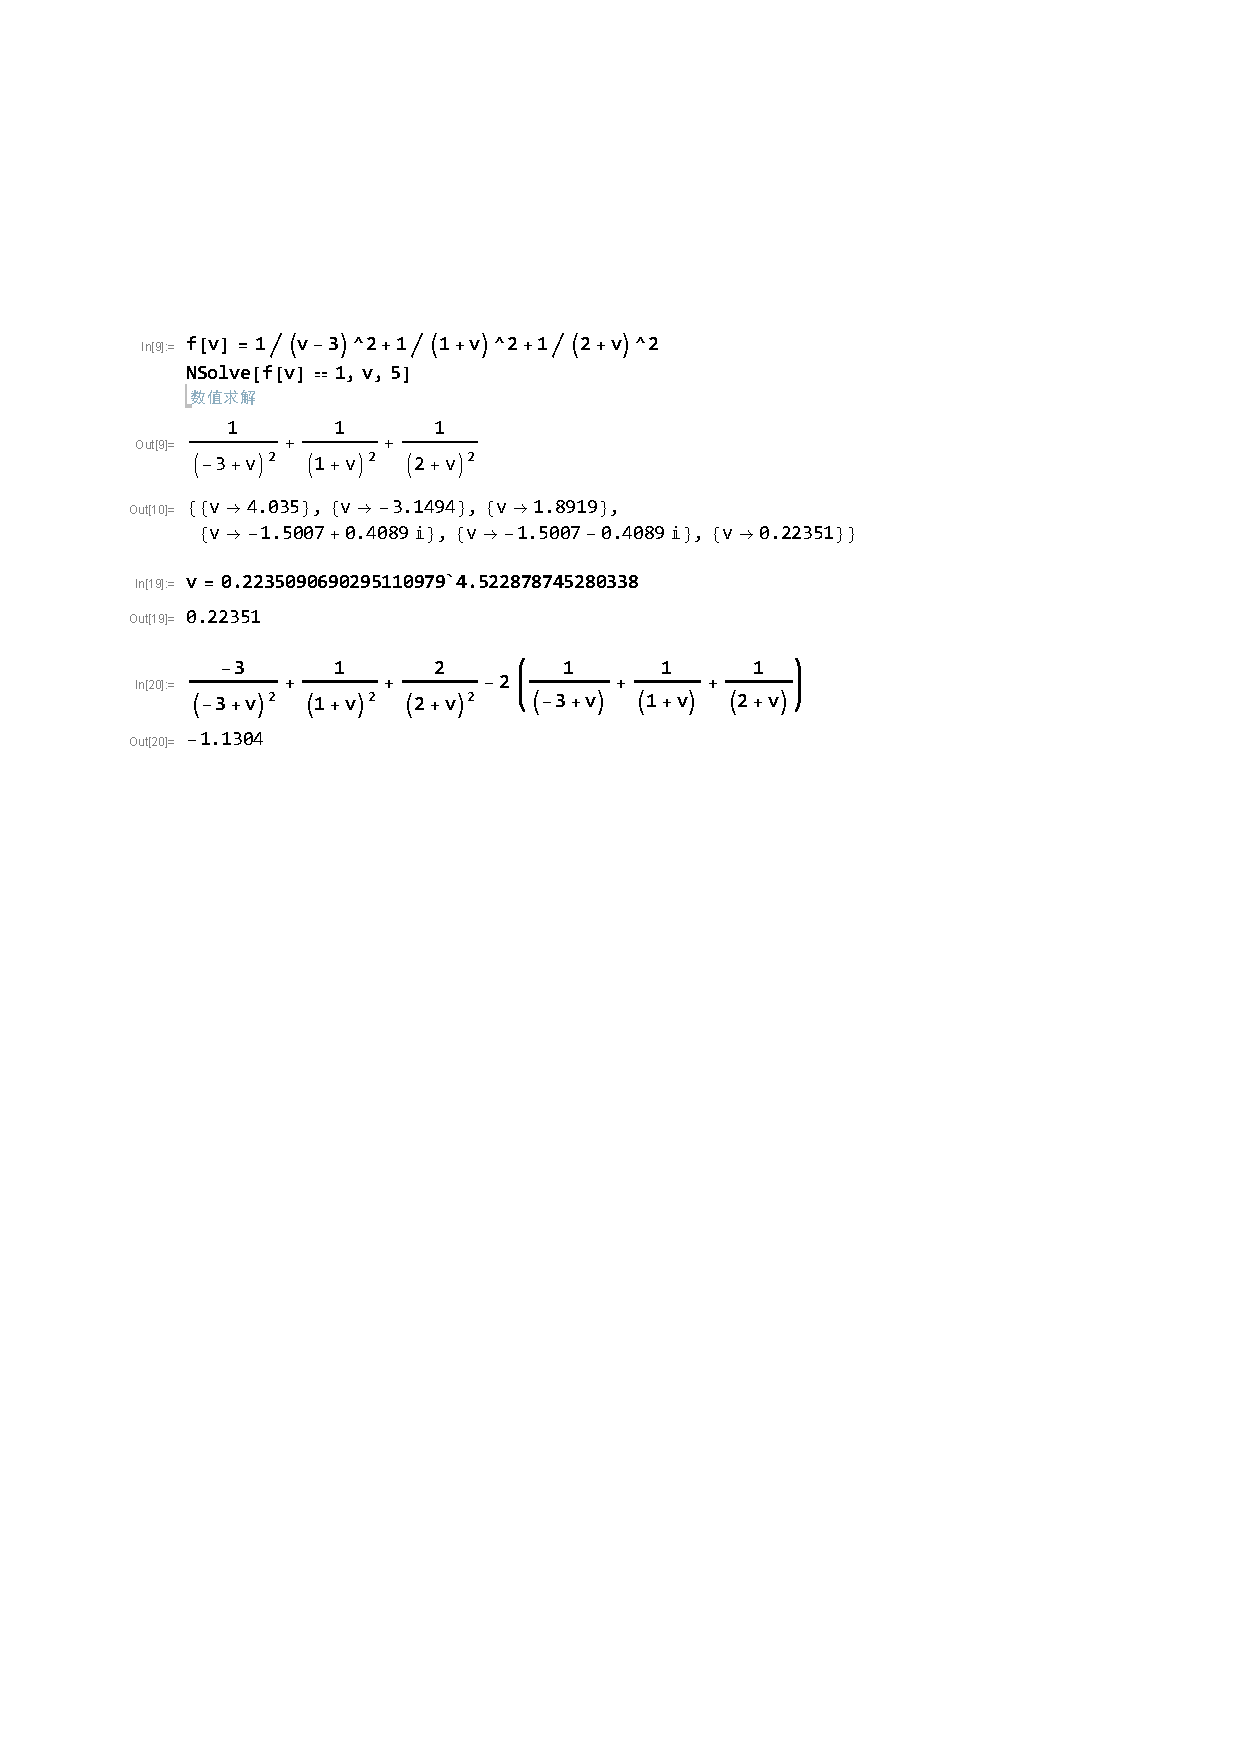
\includegraphics[scale=0.5]{p1.png}
    \caption{Solution from Gurobi, which is same to the dual problem}
\end{figure}
We can verify the solution through Gurobi package in python, and it gives the same solution hence it's strong duality.
\section*{Problem 2}
Consider the following problem
\begin{eqnarray*}
\min_{x,z,\xi,\rho} & & \frac{1}{2} x^\top x - \nu \xi + \frac{1}{m} \sum_{i=1}^m\nolimits \rho_i \\
\mathrm{s.t.} & & b_i (x^\top \phi(a_i) + z) \geq \xi - \rho_i, \forall i = 1, 2, \ldots, m\\
& & \xi \geq 0, \rho_i \geq 0, \forall i = 1, 2, \ldots, m,
\end{eqnarray*}
and denote its optimal solution as $x^*, z^*, \xi^*, \rho^*$.

You are asked to prove that $\nu$ is an upper bound on the fraction of margin errors, i.e., the number of samples falling in the margin is less than $\nu m$:
\[
\#\{i: b_i f^*(a_i) < \xi^* \} \leq \nu m,
\]
where $f^*(a) = {x^*}^\top \phi(a) + z^*$

{\bf{Answer.
Aaccording to the process for SVM:
$$L(x,z,\rho,\xi,\lambda,v,u)=\frac{1}{2}x^Tx-\nu\xi+\frac{1}{m}\sum_i^m\rho_i+\sum_i^m\lambda_i(\xi-\rho_i-b_i(x^\top\phi(a_i)+z))-\sum_i^mv_i\rho_i-u\xi$$
Then for the original problem, our object becomes:
$$\min_{x,z,\rho,\xi}\max_{\lambda_i,v_i,u}\frac{1}{2}x^Tx-\nu\xi+\frac{1}{m}\sum_i^m\rho_i+\sum_i^m\lambda_i(\xi-\rho_i-b_i(x^\top\phi(a_i)+z))-\sum_i^mv_i\rho_i-u\xi$$
s.t. $$\lambda_i,v_i,u\geq0,\forall i$$
We can first calculate the minimization problem through gradient:
$$\frac{\partial L}{\partial x}=0\rightarrow x=\sum_i^m\lambda_ib_i\phi(a_i)$$
$$\frac{\partial L}{\partial z}=0\rightarrow \sum_i^m\lambda_ib_i=0$$
$$\frac{\partial L}{\partial \rho}=0\rightarrow v_i=\frac{1}{m}-\lambda_i$$
$$\frac{\partial L}{\partial \xi}=0\rightarrow \sum_i^m\lambda_i=u+\nu$$
Plug it back we get:
$$\max_{\lambda_i}-\frac{1}{2}\sum_j^m\sum_i^m\lambda_ib_i\phi(a_i)\phi(a_j)b_j\lambda_j$$
s.t. $$\frac{1}{m}\geq\lambda_i\geq0,\forall i$$
$$\sum_i^m\lambda_ib_i=0$$
$$\sum_i^m\lambda_i\geq \nu$$
For the KKT condition we have:
$$\left\{\begin{array}{c}
    \lambda_i,v_i,u_i,\rho_i\geq0,\xi\geq0,\forall i\\
    b_i(x^\top\phi(a_i)+z)+\rho_i-\xi\geq0\\
    \lambda_i(\xi-\rho_i-b_i(x^\top\phi(a_i)+z))=0\\
    u\xi=0\\
    \sum_i^mv_i\rho_i=0
\end{array}\right.$$
Assume $n=\#\{i: b_if(a_i)<\rho\},\text{ for them } \xi=\rho-b_if(a_i)>0\rightarrow u=0\rightarrow \nu=\sum_i^m\lambda_i\geq\frac{n}{m}$
\\Hence, $\nu\text{ is the upper bound for }n$, which is the fraction of margin errors.
}}

%%%%%%%%%%%%%%%%%%%%%%%%%%%%%%%%%%%%%%%%%%%%%%%%%%%%%%%%%%%%%%%%%%%%
% Reference
%%%%%%%%%%%%%%%%%%%%%%%%%%%%%%%%%%%%%%%%%%%%%%%%%%%%%%%%%%%%%%%%%%%%
\newpage
\section*{Python Code for P1}
\begin{verbatim}
    from gurobipy import *
    WW = Model()
    WW.Params.NonConvex = 2
    s = WW.addVars(3,lb=-GRB.INFINITY, ub=GRB.INFINITY, vtype='C', name="x") # m sets
    WW.setObjective(-3*s[0]*s[0]+s[1]*s[1]+2*s[2]*s[2]+2*(s[0]+s[1]+s[2]), GRB.MINIMIZE)
    WW.addQConstr(s[0]*s[0]+s[1]*s[1]+s[2]*s[2]==1)
    WW.optimize()
    print('s=',WW.getAttr('X',s).values())
\end{verbatim}
\section*{Mathematica Code for P1}
\begin{figure}[H]
    \centering
    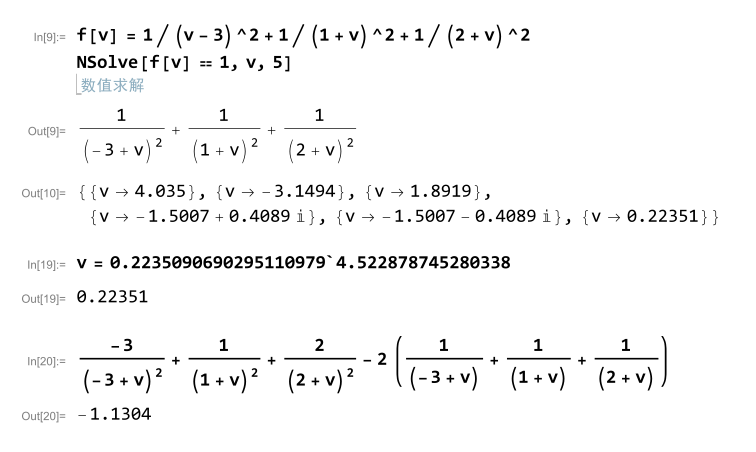
\includegraphics[scale=1]{Code.png}
    \caption{Mathematica Code to solve root for $v$ in P1}
\end{figure}
\end{document}

